\section{Blast Algorithm}
\label{sec:blast}

\begin{figure}[t!]
\centering
	\begin{subfigure}[]
    \centering
    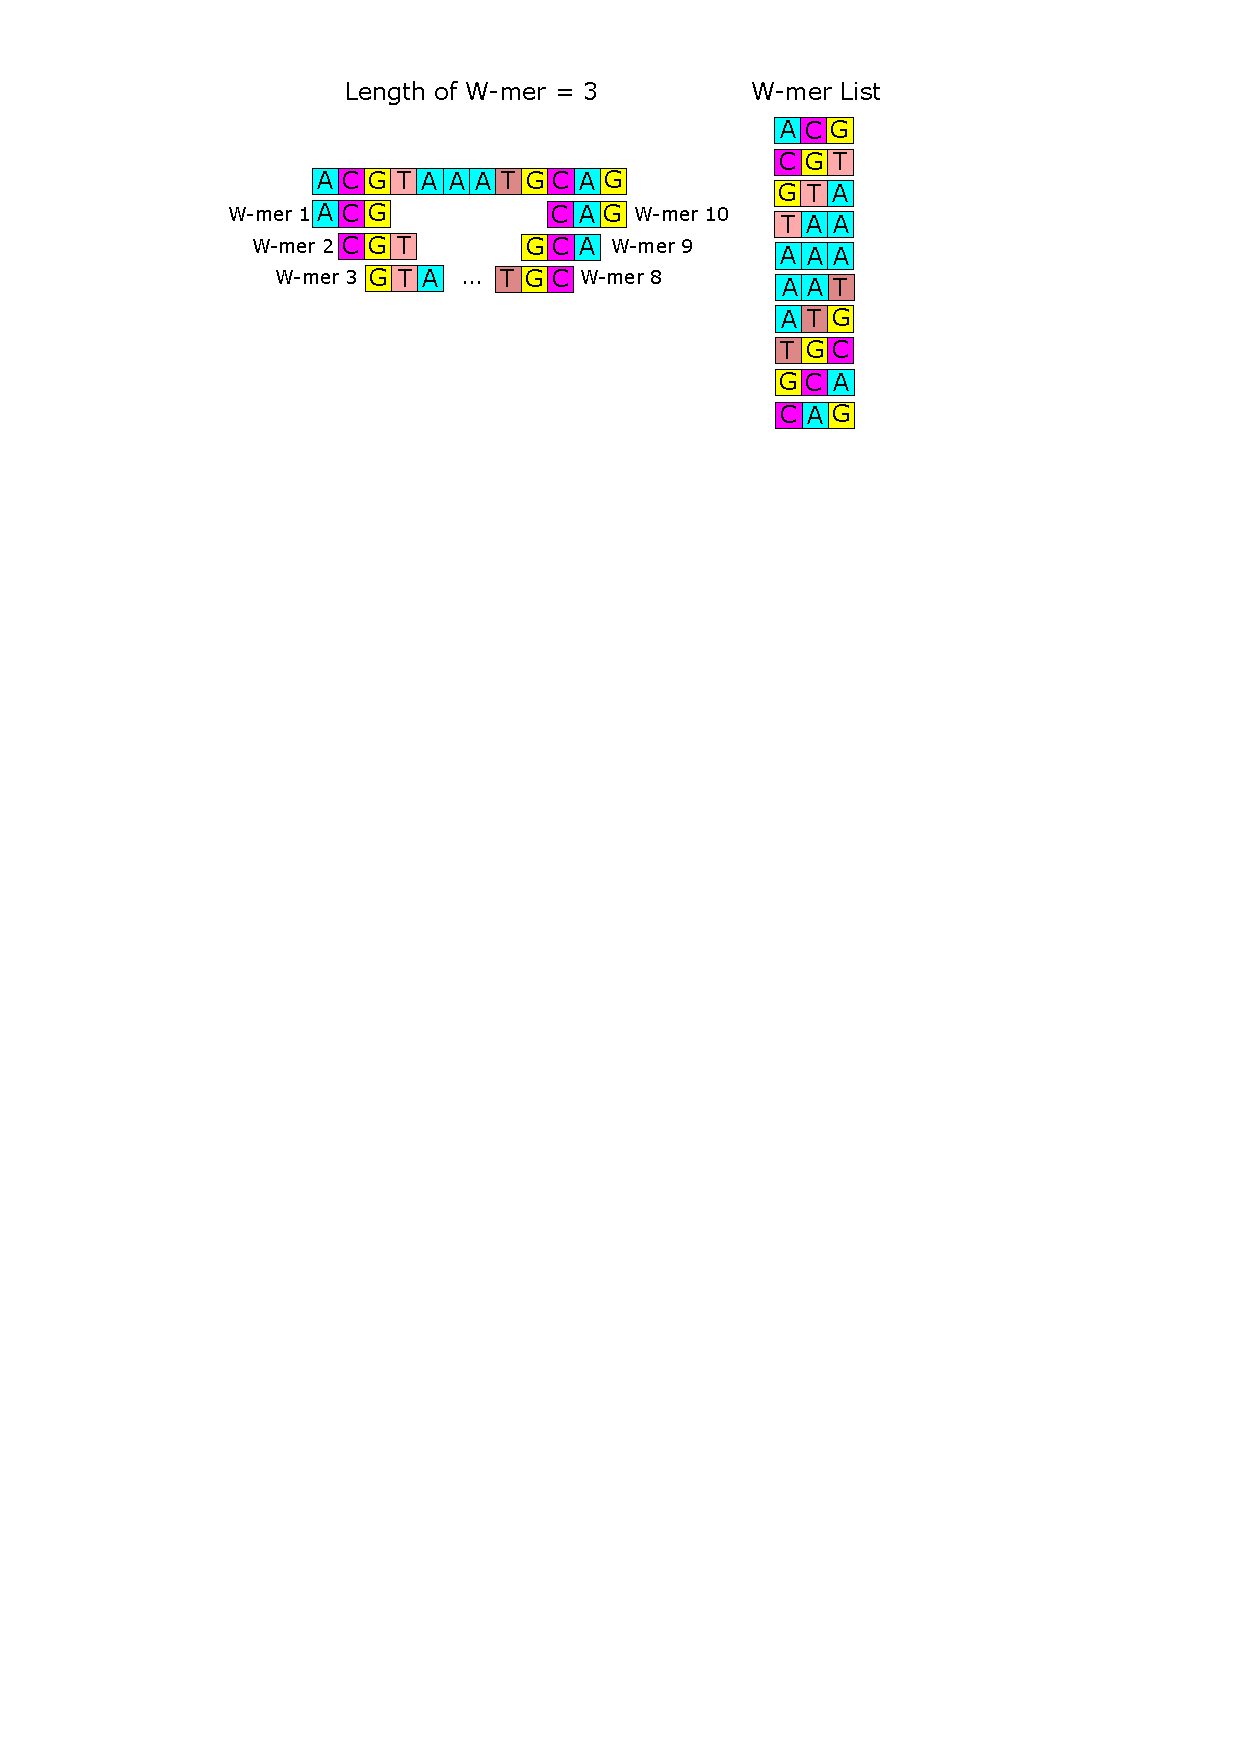
\includegraphics[width=\columnwidth]{Figures/Algorithm1.pdf} 
    \end{subfigure}
	\begin{subfigure}[]
    \centering
    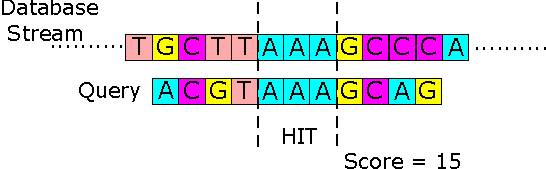
\includegraphics[width=\columnwidth]{Figures/Algorithm2.pdf}
	\end{subfigure}
	\caption{(a)~Finding W-mers from a query by creating substrings of size 3, (b)~Example of exact match between a querry and a database sequence}
	\label{fig:step12}
\end{figure}

BLAST algorithm is used to search for similar parts of sequences in a database and a query~\cite{Stephen1990}. 
Both the database and querry sequences are represented using strings of English alphabet with each letter representing a nucleobase such as Adenine, Thymine etc.
There are multiple implementations of BLAST based on the type of data they process. 
DNA sequence search uses nucleotides with 4-letter  representation and protein search uses amino acids with 20-letter representation. 
The input to BLAST are two sequences; a database, which consists of a large amount of classified data such as known viral DNAs, and a query, such as a piece of unknown DNA, which has to be compared with the database and find the similar parts. 
The output of the algorithm are the degree~(score) of similarity of the aligned parts and their corresponding location in the sequences. 
Each matched pair between the database and the query is called a High Score Pair~(HSP) and is of extreme importance for further biological computations. 
BLAST algorithm consists of 3 primary steps:
\begin{itemize}
\item{\textit{Pre-processing the query sequence}. The query is divided into several small portions/words.} 
\item{\textit{Searching for hit}. Obtained small words of query are compared to the data in database to determine the exact match.}
\item{\textit{Expansion of comparison around hits}. Locations where the sequences coincide, the comparison is continued to both sides and HSP is calculated.}
\end{itemize}
Details of each step is discussed in detail below.

\subsection{Pre-processing}
In this step, a query is divided into a list of substrings, as shown in Fig.~\ref{fig:step12}~(a). 
These substrings are called W-mers of length W~\cite{sotiriades2007design}. 
Let us assume we have a query DNA sequence ACGTAAARGCAG of length 12 and W-mers of length 3 \cite{sotiriades2007design}. 
Since the W-mers are contiguous substrings, there are in total 10 W-mers. 
The total number of W-mers in a querry can be calculated as 
\begin{equation}
\label{eq1}
No.of \ Wmers = Query \ Length - Wmer \ Length + 1 
\end{equation}
The substring ACG will be the first W-mer, CGT the second and so on. 



\subsection{Searching for hits}
After the query is divided and the list of W-mers is generated, the search for exact match between W-mers and database is conducted.
W-mers are chosen and randomly compared with the portions of the database. 
Every exact match found is recorded as a ``hit" and saved to process further in step 3 as shown in Fig.~\ref{fig:step12}~(b). 


\subsection{Expansion}
After sufficient number of hits are found, each W-mer with exact match is expanded locally to both directions (left and right) by single letter per direction at a time as shown in Fig.~\ref{fig:step3}. 
The expansion continues until the scoring no longer gets improved.
\begin{figure}[t!]
\centering
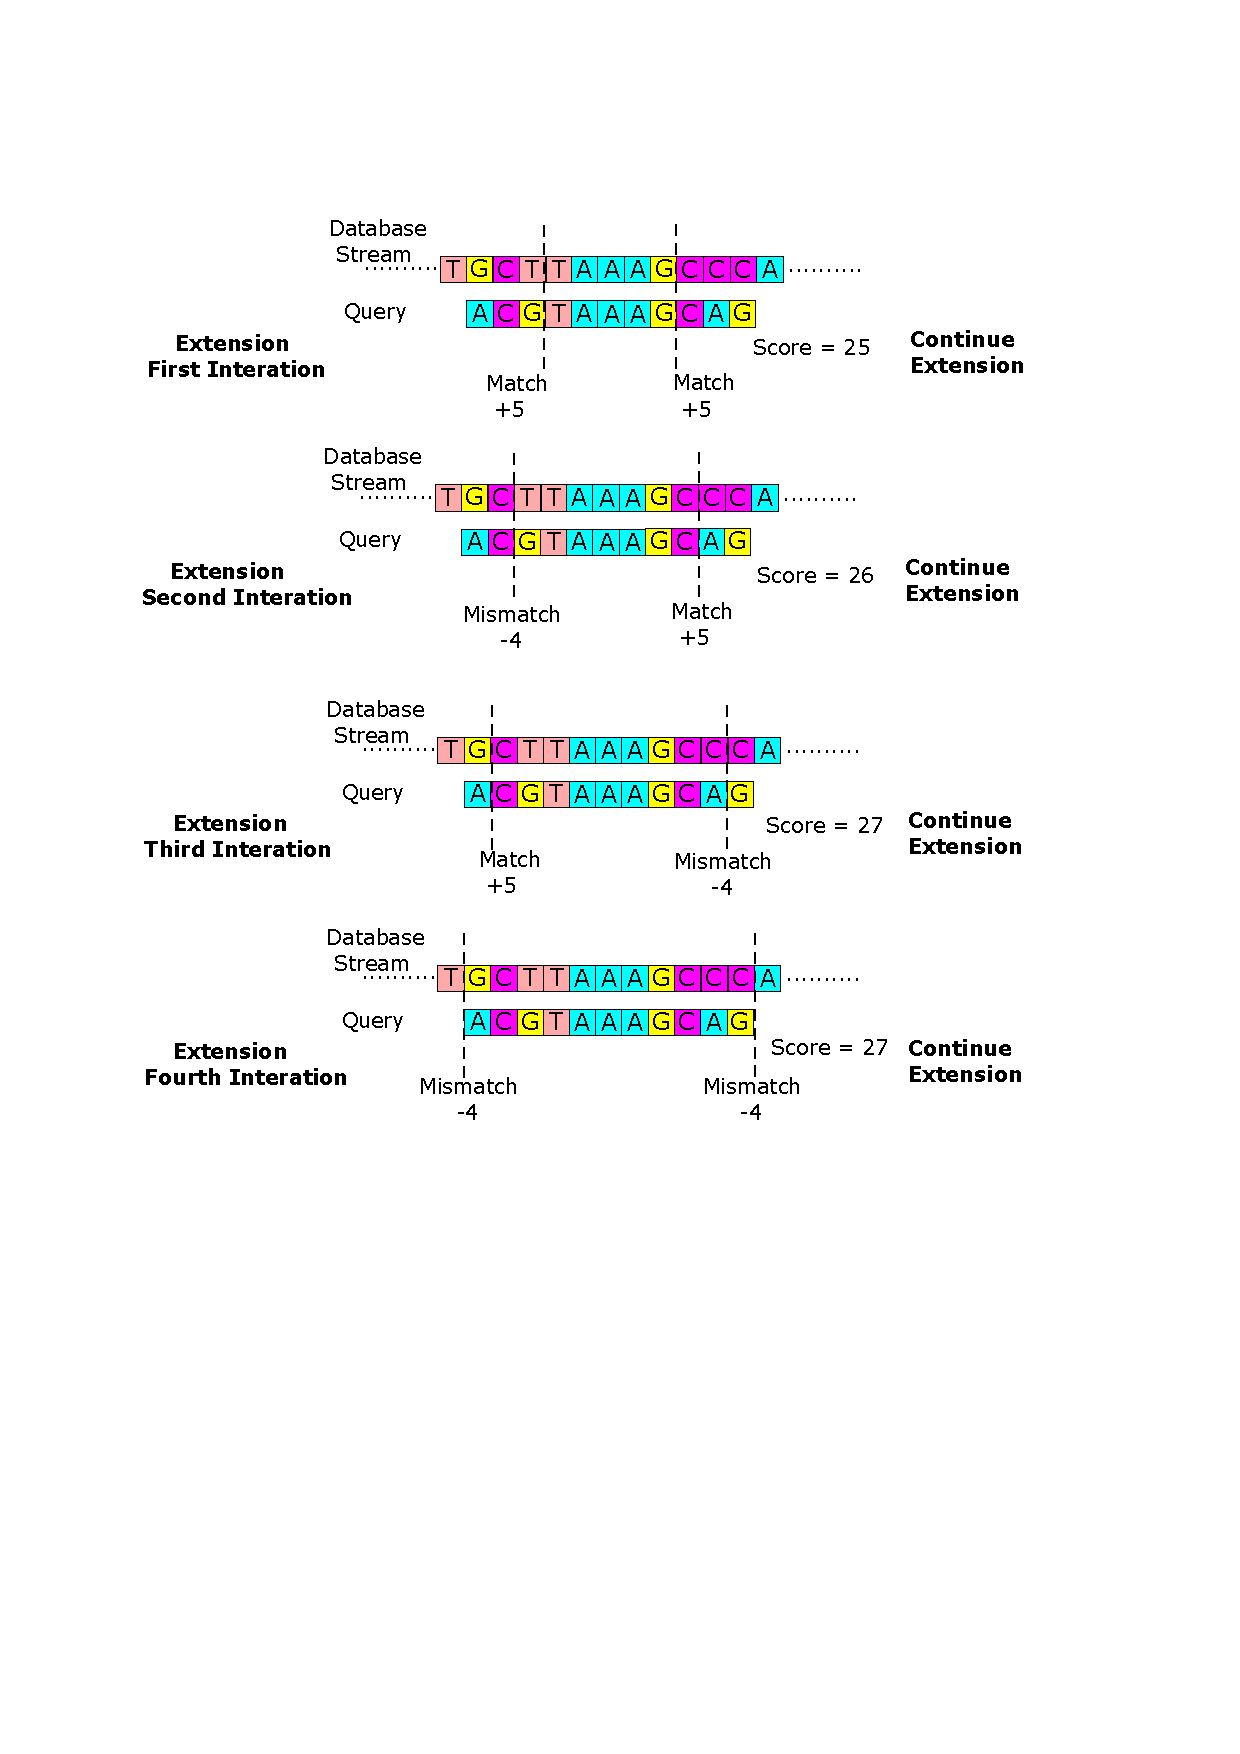
\includegraphics[width=\columnwidth]{Figures/Algorithm3.pdf}
\caption{Example of BLAST Algorithm's Third Step: Expansion of Comparison around Hits} 
\label{fig:step3}
\end{figure}
The scoring technique of the algorithm is based on the Point Accepted Mutations~(PAM) matrices, that are used to examine which amino-acid substitutions are biologically accepted~\cite{sotiriades2007design}. 
However, due to the complexity of this technique, a simpler and biologically acceptable scoring method is generally used. 
In the expansion stage, each new match will results in addition of 5 points to the score and any mismatch will lead to reduction of 4 from the score as depicted in Fig.\ref{fig:step3}.
The expansion ceases when the score calculated after an expansion becomes less than the score before expansion.
The substrings with maximum score are selected and are called HSPs.
The HSPs and the correponding score are reported as the final output of the algorithm.

